\documentclass{article}   
\usepackage[utf8]{inputenc}

\usepackage{color}
\usepackage{graphicx} % in the STTT example
\usepackage{amsmath}
\usepackage{amssymb}
\usepackage{mathtools}
\usepackage{algorithm}
\usepackage{multirow}
\usepackage{color}
%\usepackage{amsmath,amssymb,dsfont}
\usepackage{multirow}
\usepackage{algpseudocode}
\usepackage{algorithmicx}
\usepackage{dblfloatfix}

\renewcommand{\textfraction}{0.05}
\renewcommand{\floatpagefraction}{0.90}


\newcommand{\red}[1]{\textcolor{red}{#1}}
\newcommand{\blue}[1]{\textcolor{blue}{#1}}

\newcommand{\IGNORE}[1]{}

\newcommand{\ttit}[1]{{\text{\it #1}}}
\newcommand{\imgchar}[1]{{\bf\small({#1})}}
%\newcommand{\rewrite}{Rewrite}
\newcommand{\Sat}{\text{\it Sat}}
\newcommand{\SatELTL}{\text{Sat{$\exists$}LTL}}
\newcommand{\SatLTL}{\text{SatLTL}}
\newcommand{\SatCTL}{\text{SatCTL}}
\newcommand{\SatCTLstar}{\text{SatCTL*}}
\newcommand{\satCTL}{\Call{satCTL}}
\newcommand{\satLTL}{\Call{satLTL}}
\newcommand{\satELTL}{\Call{sat{$\exists$}LTL}}
\newcommand{\rewrite}{\Call{rewrite}}
\newcommand{\tuple}[1]{{\langle{#1}\rangle}}
\newcommand{\CTLstarMEDD}{{\small RGMEDD*}}
\newcommand{\RGMEDD}{{\small RGMEDD3}}
\newcommand{\ltsmin}{LTSmin}
\newcommand{\greatspn}{GreatSPN}
\newcommand{\meddly}{Meddly}
\newcommand{\spot}{Spot}
\newcommand{\Paths}{\mathbf{\cal P}}
\newcommand{\place}[1]{#1}
\newcommand{\trans}[1]{#1}
\newcommand{\Lang}{\mathcal L}
\newcommand{\AP}{AP}


\newcommand{\PsiRule}{\boldsymbol\Psi}
\newcommand{\phiRule}{\boldsymbol\phi}
\newcommand{\varphiRule}{\boldsymbol\varphi}
\newcommand{\doubleAmp}{\ensuremath{\mathop{\scalebox{0.80}{\&\!\&}}}}
\newcommand{\doublePipe}{\ensuremath{\mathop{\scalebox{0.80}{$||$}}}}

\begin{document}
\title{Esercizio Reti di Petri Produttori e Consumatori}
\author{Ruben Castelluccio}



   
 
\date{\today}

\maketitle
\section{Introduzione}
L'esercizio consiste nell'Analisi mediante Reti di Petri per il problema Produttore - Consumatore.
\\ Si richiede di analizzare 3 diversi modelli di Produttore e Consumatore dove il Buffer è sempre definito a N posizioni:
\begin{itemize}
    \item Primo Setting: 1 Produttore, 1 Consumatore, Buffer a N posizioni;
    \item Secondo Setting: 1 Produttore, 2 Consumatori, Buffer a N posizioni;
    \item Terzo Setting: P Produttori, C Consumatori, Buffer a N posizioni.
    \end{itemize}
    E' richiesto per il Setting 2 e Setting 3 di implementare 2 diverse soluzioni: basata sulla marcatura e basata sulla replicazione.
    \\\\Inoltre si richiede per ciascun Setting il Modelling Convenience, valutazione della difficoltà dell'implementazione e la Solution Convenience, dove si confronta il RG del Setting 2 e Setting 3.
    
\clearpage
\section{Primo Setting}
Nel Primo Setting è richiesta la Rete di Petri per lo schema Produttore e Consumatore in cui è presente: 1 Produttore, 1 Consumatore e Buffer a N posizioni.
\\\\Il Produttore è definito da una posto iniziale P0 da cui si può far scattare la transizione \textit{P\_Think} per andare nel posto P1 che farà scattare la transizione \textit{Produce} che inserisce un token nel posto P2 e abilita la transizione \textit{Put}, se è presente almeno un token nel posto \textit{BufferLiberi}, inserendo un token nel posto \textit{BufferOccupato} e un token nel posto iniziale P0 permettendo in questo modo al Produttore di poter tornare a pensare e produrre.
\\\\Il Consumatore è definito da un posto iniziale C0 in cui sarà in attesa che la transizione \textit{Get} possa essere abilitata, cosi facendo prenderà un token dal Buffer portando un token nel posto \textit{BufferLiberi} e un token nel posto C1, dopodichè farà scattare la transizione \textit{C\_Think} e andrà nel posto C2, successivamente facendo scattare la transizione \textit{Activity} tornerà nel posto iniziale C0.



\begin{figure}[h] 
\centering
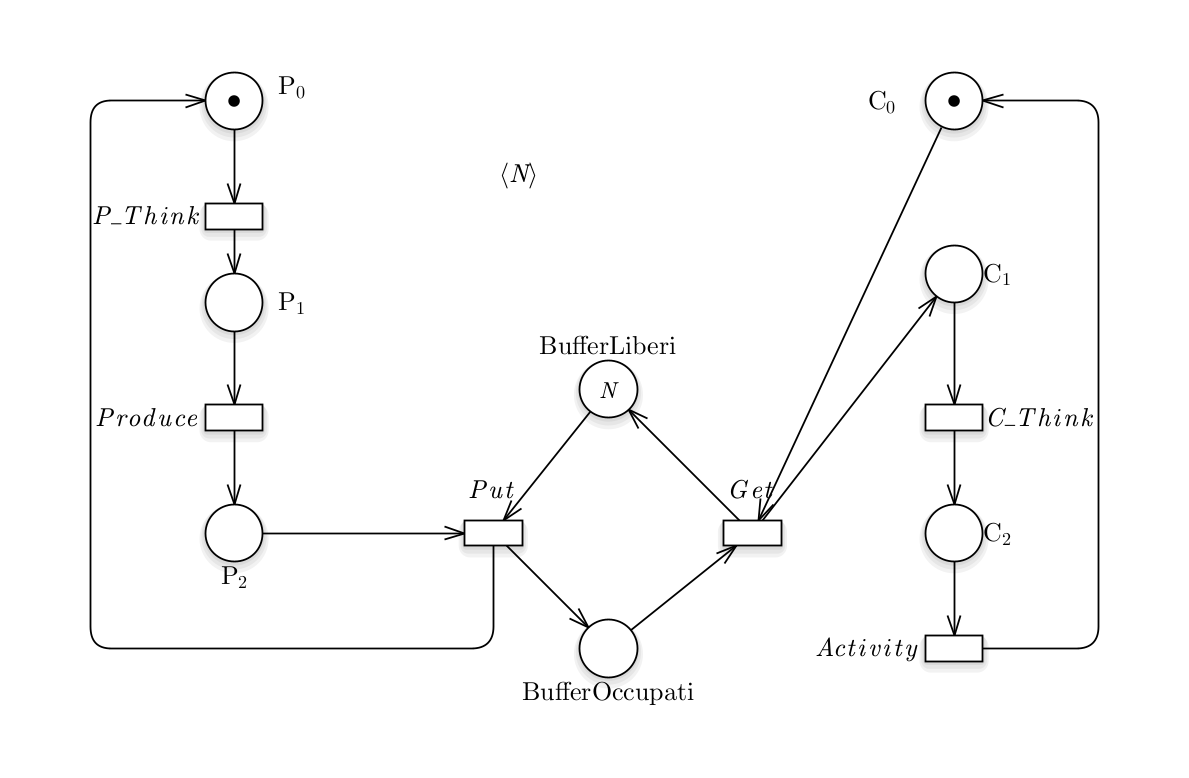
\includegraphics[scale=0.3]{PT-Setting 1.png}
\end{figure}
\subsection{Modelling Convenience}
L'implementazione del Primo Setting non ha generato difficoltà essendo stato commentato e illustrato a lezione.
\clearpage
\section{Secondo  setting}
Nel Secondo Setting è richiesta la Rete di Petri per lo schema Produttore - Consumatore in cui sono presenti: 1 Produttore, 2 Consumatori e Buffer a N posizioni. Sono richieste 2 diverse implementazioni: scalatura su Marcatura e scalatura su Replicazione
\subsection{Secondo  Setting: Scalatura per Marcatura}
Nell'implementazione Scalatura per Marcatura, a differenza del Setting 1, si aggiunge un ulteriore Consumatore mediante la costante \textit{C} impostata a 2 modificando pertanto la marcatura iniziale del posto \textit{C0}. 
\begin{figure}[h] 
\centering
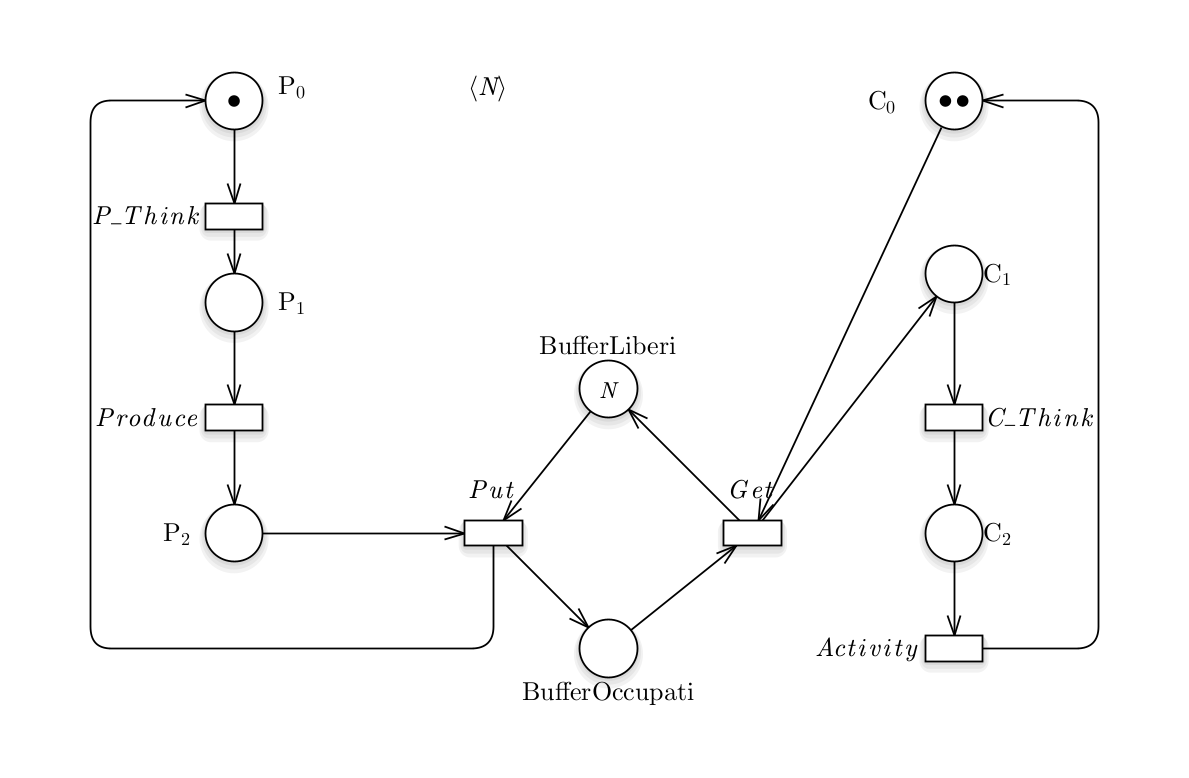
\includegraphics[scale=0.4]{setting2marcaturaPT.png}
\end{figure}

\subsection{Secondo  Setting: Scalatura per Replicazione}
Nella Scalatura per Replicazione si duplica la struttura del consumatore, in particolare avremo 2 transizioni \textit{Get} affinchè i 2 consumatori possano prelevare il Token dal posto \textit{BufferOccupati} in modo indipendente.
\begin{figure}[h] 
\centering
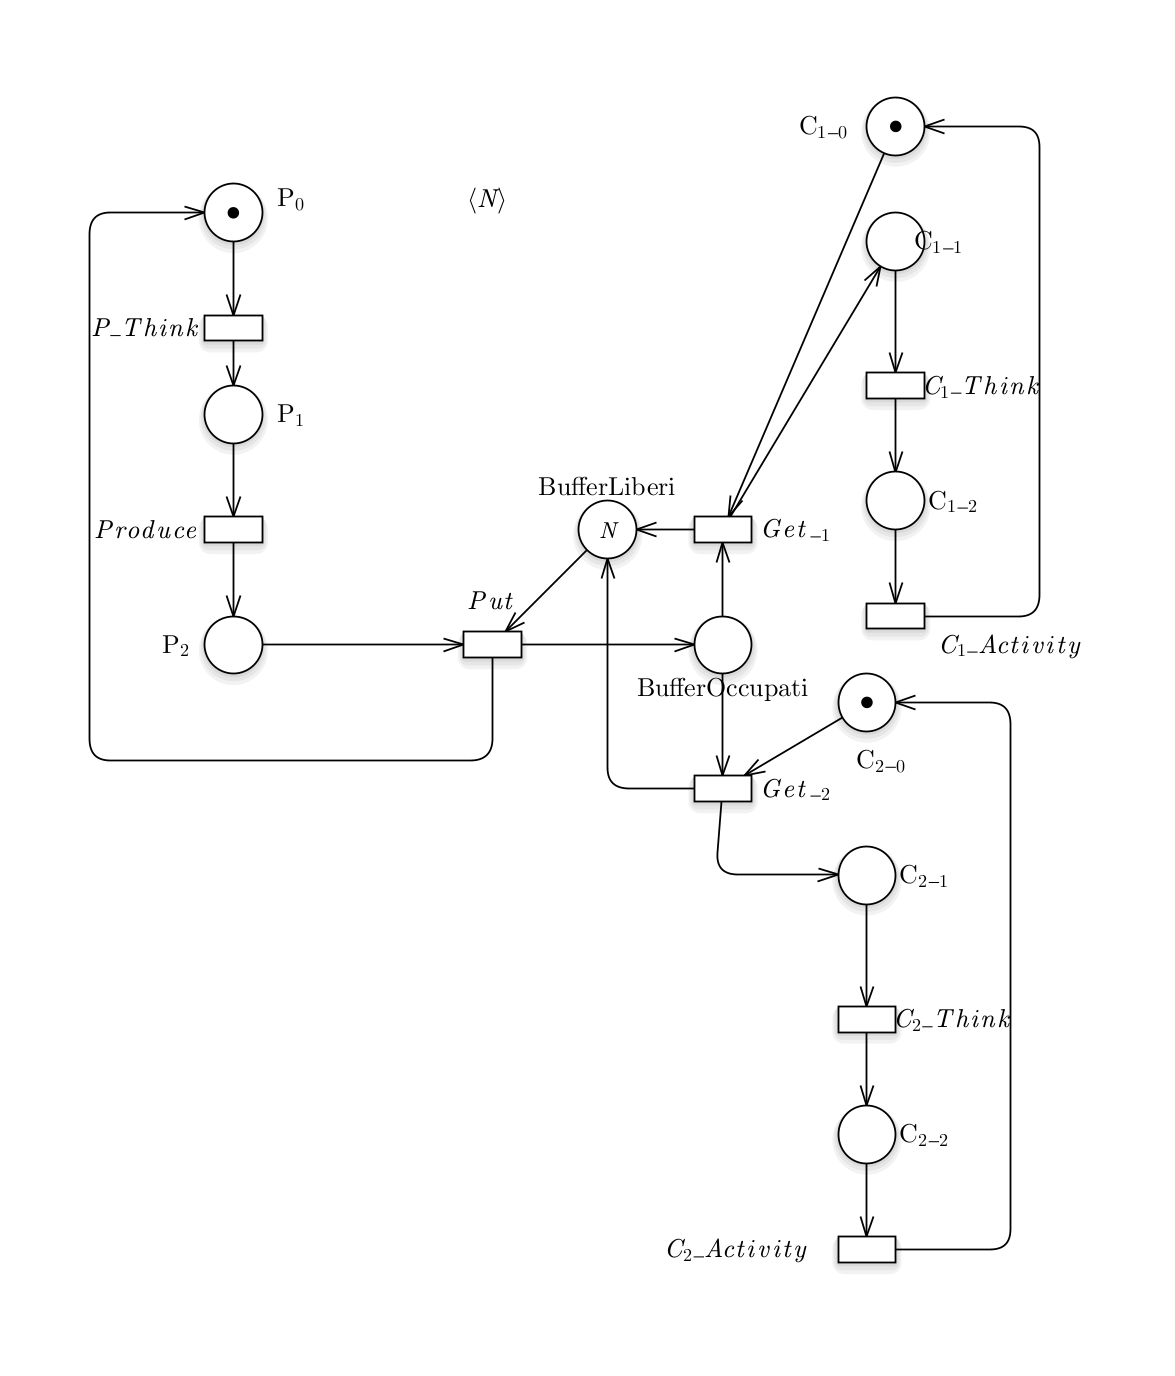
\includegraphics[scale=0.4]{PT-Setting2 - Replicazione.png}
\end{figure}
\clearpage
\subsection{Modelling Convenience}
La difficoltà significativa riscontrata per l'implementazione del Setting 2 ha riguardato la Scalatura per Replicazione dato che si è dovuto adattare il Buffer non più a un solo Consumatore ma a 2 affinchè accedessero in maniera del tutto indipendente. Pertanto, oltre la duplicazione dell'intera struttura del Consumatore, è stato richiesto di implementare 2 differenti transizioni \textit{Get} che collegassero il Buffer ai Consumatori.
\subsection{Solution Convenience}
Nella Solution Convenience è richiesto di confrontare i Reachability Graphs della Scalutara per Marcatura e Scalatura per Replicazione. Il numero di Token nel buffer è pari a 2.
\\Dalle verifiche effettuate è risulato che il numero di marcature nell'approccio della Scalatura per Marcatura è pari a 54 mentre nella Scalatura per Replicazione se ne sono ottenute 82.
\\Pertanto nell'approccio che prevede la duplicazione del Consumatore si evidenzia un Reachability Graph con un numero di marcature piu elevato rispetto alla Scalutura per Marcatura.

\clearpage
\section{Terzo  Setting}
Nel Terzo Setting è richiesta l'implementazione di una Rete di Petri per il problema Produttore - Consumatore in cui sono presenti: P Produttori, C consumatori e il Buffer a N posizioni.
\\Si è deciso di stabilire 2 Prdouttori e 2 Consumatori al fine di ottenere 2 differenti implementazioni, analogamente a quanto avvenuto con il Setting 2: Scalatura per Marcatura e Scalatura per Replicazione.
\subsection{Terzo  Setting: Scalatura per Marcatura}
In maniera del tutto analoga a quanto avvenuto per il Setting 2, in quest'approccio, la struttura della rete rimane invariata con eccezzione per la modifica nei posti iniziali, sia per il Produttore sia per il Consumatore, definiti entrambi da costanti parametriche.

\begin{figure}[h] 
\centering
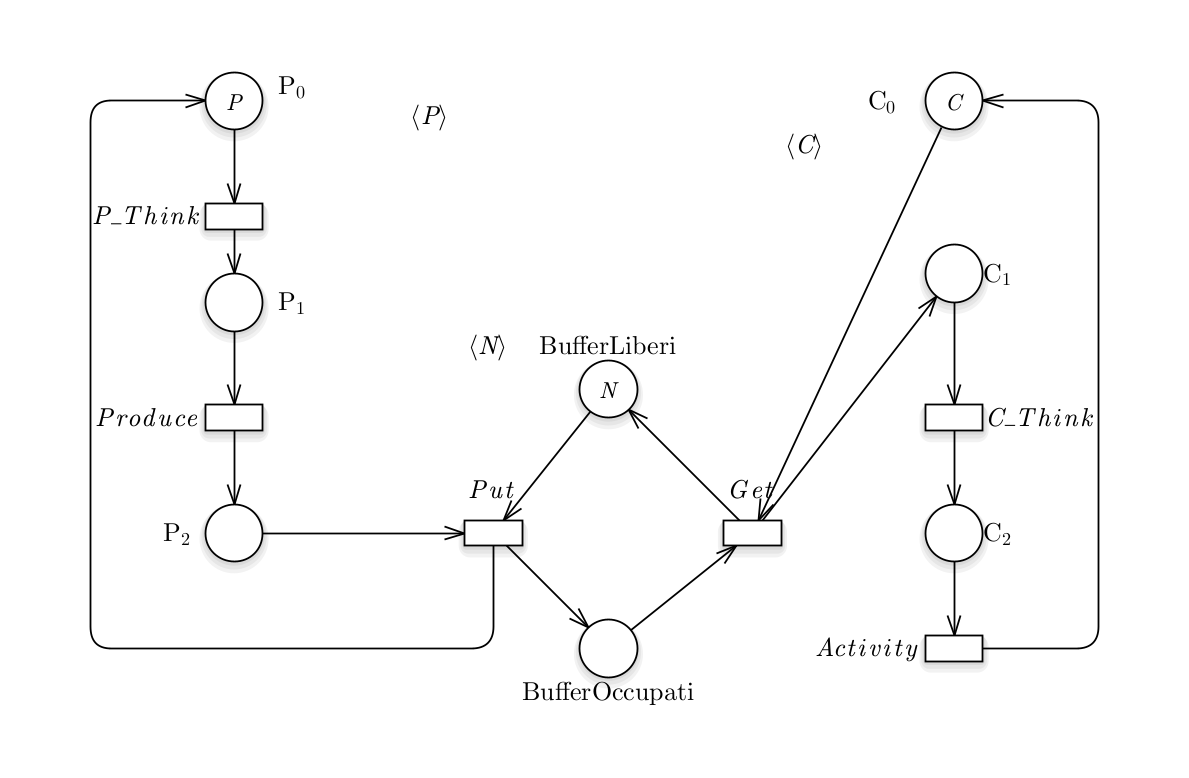
\includegraphics[scale=0.3]{PT-Setting 3 - Marcatura.png}
\end{figure}
\subsection{Terzo  Setting: Scalatura per Replicazione}
Per il Terzo Setting, nell'approccio Scalatura per Replicazione, rispetto al Secondo Setting, si è duplicata la struttura del Produttore, ottenendo pertanto una rete composta da 2 Produttori e 2 Consumatori. In maniera del tutto speculare cosi come i Produttori possono produrre e inserire nel Buffer, presupponendo di avere token nel posto \textit{BufferLiberi} per abilitare la transizione \textit{Put}, anche i Consumatori potranno prelevare dal Buffer in maniera indipendente i Token nel posto \textit{BufferOccupati} mediante la transizione {Get}.
\begin{figure}[h] 
\centering
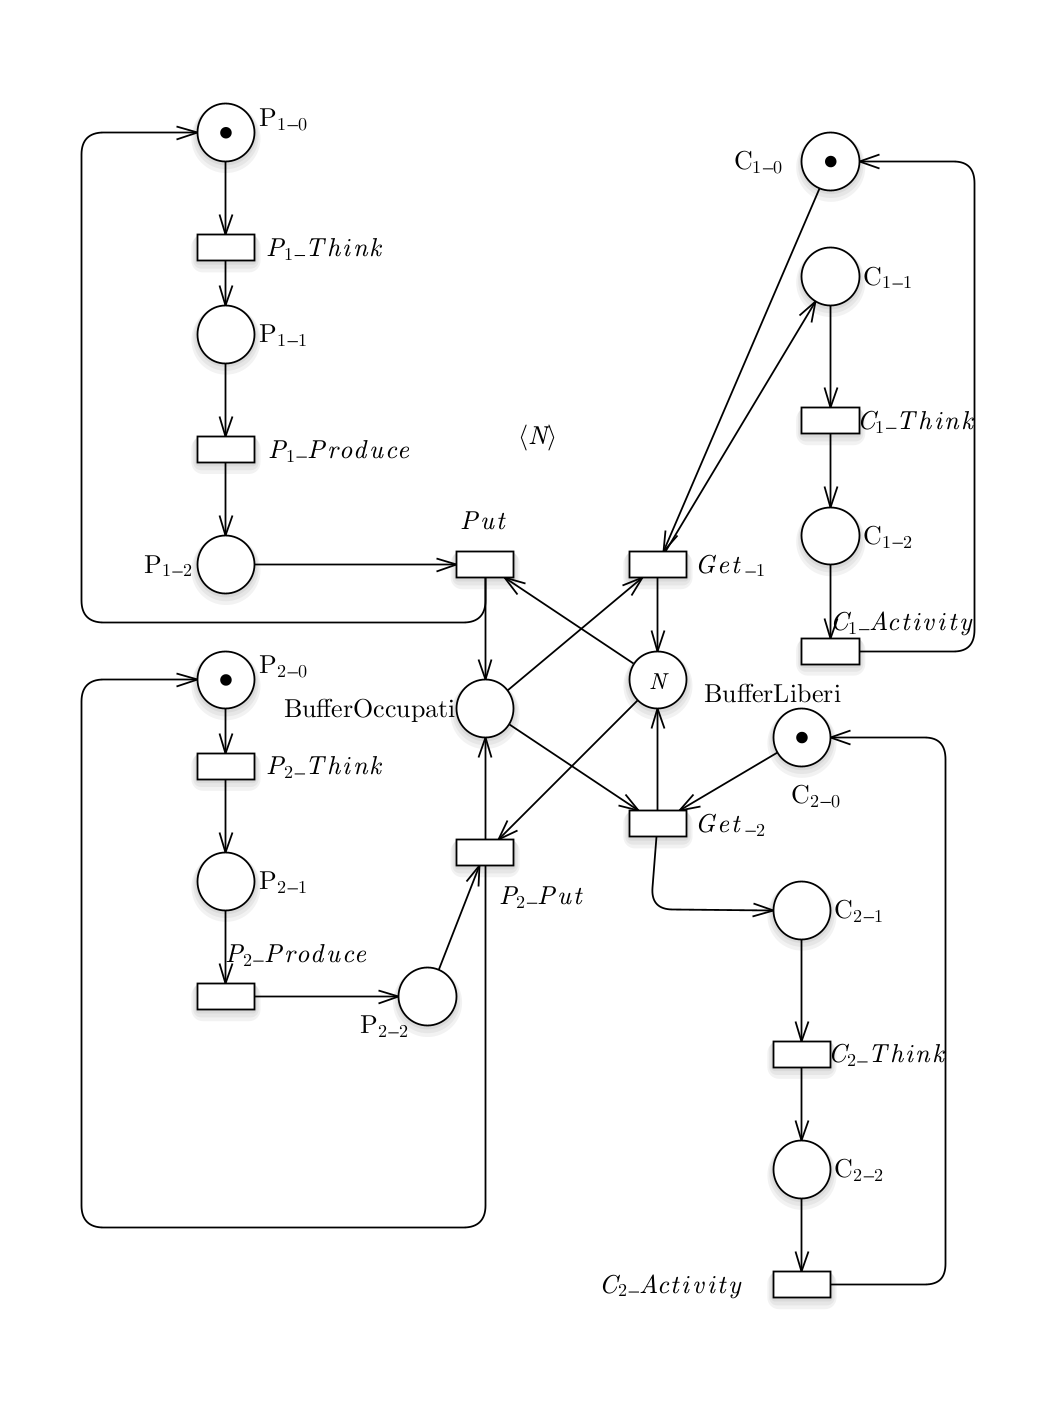
\includegraphics[scale=0.4]{PT-Setting3- Replicazione.png}
\end{figure}
\clearpage
\subsection{Modelling Convenience}
In questo Setting, la difficoltà principale è stato l'adattamento, per la Scalatura per Replicazione, di un secondo Produttore alla rete, con particolare attenzione alla transizione \textit{Put} e gli archi per collegarla ai posti del Buffer: \textit{BufferOccupati} e \textit{BufferLiberi}.
\subsection{Solution Convenience}
Per la generazione dei Reachability Graphs di entrambi gli approcci sono state assegnati i seguenti valori:
\begin{itemize}
    \item Numero Produttori: 2;
    \item Numero Consumatori: 2;
    \item Numero di Token nel Buffer: 2.
\end{itemize}
Per la Scalatura di Marcatura viene generato un Reachability Graph di 243 marcature mentre per la Scalatura di Replicazione viene generato un Reachability Graphs di 108 marcature.
\\Come evidenziato nella Solution Convenience del Setting 2, anche nel Setting 3, risulta come il numero generato nell'approccio della duplicazione della struttura Produttore e Consumatore si ottenga un numero di marcature notevolmente piu elevato.
\end{document}